\documentclass[11pt]{article}

\usepackage[T1]{fontenc}
\usepackage[utf8]{inputenc}
\usepackage{lmodern}
\usepackage[margin=1in]{geometry}
\usepackage{graphicx}
\usepackage{booktabs}
\usepackage{longtable}
\usepackage{array}
\usepackage{caption}
\usepackage{hyperref}
\usepackage{microtype}
\usepackage{seqsplit}
\usepackage{xcolor}

\setlength{\emergencystretch}{2em}

\hypersetup{
  colorlinks=true,
  linkcolor=black,
  citecolor=black,
  urlcolor=blue
}

\newcommand{\braindough}{\textsc{Braindough}}
\newcommand{\tribe}{TRIBE v2}
\newcommand{\runid}{\texttt{\seqsplit{20260516T230219131728Z-local-tribe-v2-first-suite-tribe-v2-eac66ffd}}}
\newcommand{\meanabs}{0.102670}
\newcommand{\responsevertices}{20{,}484}
\newcommand{\hemivertices}{10{,}242}
\newcommand{\runcommit}{\texttt{\seqsplit{ad146aba73d01a6f197f6f2a508c800651406d5f}}}
\newcommand{\confighash}{\texttt{\seqsplit{f4c69bbd3dac5c428b80ee83529ea6c5d0fe985432c5fbe982b75036460ae7de}}}
\newcommand{\responsehash}{\texttt{\seqsplit{5fbbf8041325b1fcac359b52584763d77af19ef0f1ce8af6b2c41417f5054edd}}}
\newcommand{\provenancehash}[1]{\texttt{\seqsplit{#1}}}
\newcommand{\pkg}[1]{\texttt{\seqsplit{#1}}}

\title{\braindough: A Single-Run \tribe{} Predicted-Response Artifact with Vertex-Index Brain Schematic Visualization}
\author{Peyton Kadej}
\date{2026-05-16}

\begin{document}
\maketitle

\begin{abstract}
\tribe{} is a multimodal brain-encoding model that predicts average-subject
fMRI-like cortical responses to video, audio, and language stimuli. This
technical preprint reports a deliberately bounded \braindough{} run that
converts generated visual stimuli into short video events, executes one real
\tribe{} prediction, checks the resulting artifact, and adds a transparent
vertex-index brain schematic for review. The run generated 39 stimuli as
context across five suites and retained one model response for
\texttt{image\_activation:color\_gradient:static}. The response array has shape
$2 \times \responsevertices{}$, corresponding to two retained model output
segments over an fsaverage5-like cortical vertex vector; mean absolute
predicted response was \meanabs{}. Because the artifact does not include
fsaverage5 surface coordinates or an ROI atlas, the visualization uses an
explicit convention: split the vector into two \hemivertices{}-vertex halves
and project values onto a two-hemisphere schematic. The central contribution is
a reproducible local artifact and reporting pattern, not a measured
neuroscience result or spatial-registration method: all values are
model-predicted average-subject responses, the brain figure is a vertex-index
schematic rather than anatomical registration, and no subject-specific,
diagnostic, hemispheric, or ROI claim is made.
\end{abstract}

\section{Introduction}

Foundation-model approaches are beginning to make in-silico neuroscience
workflows practical on local workstations. \tribe{} is a recent tri-modal brain
encoding model for video, audio, and language that predicts fMRI-like responses
to naturalistic and experimental stimuli \cite{dascoli2026foundation}. The
public repository exposes pretrained-model loading, event extraction from
video, and predictions shaped as \texttt{(n\_timesteps, n\_vertices)}
\cite{tribev2repo}. The repository further states that predictions are for
an ``average'' subject on an fsaverage5 cortical mesh and are shifted to
compensate for hemodynamic lag \cite{tribev2repo}. The model weights are
distributed on Hugging Face under a non-commercial Creative Commons license
\cite{tribev2hf}.

\braindough{} is a local-first harness for small, reproducible brain-modeling
experiments. Its practical design constraint is that source code, configs, and
small derivative reports remain in the repository, while model weights,
datasets, caches, and run outputs live under a separate \texttt{BRAINDOUGH\_HOME}.
This separation matters for \tribe{} because the checkpoint and feature
extractors are large, local inference is slow enough to require explicit
budgets, and casual visualization can easily overstate what the model output
means.

This manuscript is a methods note for a single bounded run. It answers three
engineering and reporting questions:

\begin{enumerate}
  \item Can a clean \braindough{} checkout execute a real, capped \tribe{} run
  and produce a structurally valid artifact?
  \item Can the artifact be summarized in a reviewable HTML/PDF report without
  vendoring heavy response arrays or model weights into the repository?
  \item Can a brain diagram be added without claiming anatomical ROI mapping
  when only a \responsevertices{}-value vertex vector is
  available?
\end{enumerate}

\section{Run Artifact}

The source run is \runid{}. It was produced by the root command
\texttt{just run-tribe} from the local first-suite spec
\path{experiments/local/tribe_v2_first_suite.yaml}. The spec uses
\texttt{backend: tribe-v2}, checkpoint \texttt{facebook/tribev2}, a 50-second
event window, and \texttt{max\_predictions: 1}. That cap is intentional: the
first-suite generator creates more media than this laptop-scale local run
should fully score.

The run completed on 2026-05-16 and passed structural artifact validation with
\texttt{braindough validate}. It generated 39 stimuli across five suites. Only
the first image-activation stimulus was passed through the real \tribe{}
prediction budget; the other 38 generated stimuli are unscored run context.
Table~\ref{tab:run-summary} gives the run-level facts copied from
\texttt{metrics.json} and \texttt{response\_metrics.csv}. Artifact validation
means file, schema, and internal-consistency validation, not validation of
\tribe{} calibration, accuracy, or neuroscientific interpretation.

\begin{table}[ht]
  \centering
  \caption{Run-level summary for the source run.}
  \label{tab:run-summary}
  \begin{tabular}{ll}
    \toprule
    Field & Value \\
    \midrule
    Backend & \texttt{tribe-v2} \\
    Checkpoint & \texttt{facebook/tribev2} \\
    Generated stimuli & 39 \\
    Attempted predictions & 1 \\
    Completed model predictions & 1 \\
    Predicted stimulus & \texttt{image\_activation:color\_gradient:static} \\
    Response shape & $2 \times \responsevertices{}$ \\
    Mean absolute predicted response & \meanabs{} \\
    Mean predicted response & $-0.075532$ \\
    Standard deviation & $0.148002$ \\
    Device ladder & \texttt{mps}, then \texttt{cpu} \\
    \bottomrule
  \end{tabular}
\end{table}

\begin{figure}[ht]
  \centering
  
\includegraphics[width=0.48\linewidth]{figures/color_gradient.png}
  \caption{Generated source image converted into a short silent video for the
  retained \tribe{} prediction. The video event, not the still image directly,
  is the model input.}
  \label{fig:source-image}
\end{figure}

\section{Methods}

\subsection{Stimulus temporalization}

\tribe{} inference is event-based. For static generated images, \braindough{}
creates short silent MP4 clips and submits the video path to the \tribe{} event
extractor. This matches the public quick-start interface, which derives events
from a \texttt{video\_path} before prediction \cite{tribev2repo}. The local
first suite generated baseline image-activation videos, visual controls,
visual perturbations, temporalization variants, and audio controls. The real
prediction budget kept only the first baseline image-activation clip.

The predicted clip was generated from a deterministic 256 by 256 RGB
\texttt{color\_gradient.png} image. \braindough{} wrote an MP4 with eight
identical RGB frames, 4 frames per second, 2 seconds duration, H.264
\texttt{libx264} encoding, macroblock size 16, and imageio quality 6. The
\tribe{} backend then represented that clip as a 50-second video event before
prediction, matching the local spec's \texttt{event\_duration\_seconds: 50.0}.

\subsection{Response summarization}

The retained model-predicted response is stored externally as
\texttt{outputs/responses.npz} with index metadata in
\texttt{outputs/responses.index.jsonl}. The copied manuscript figures summarize
that response without committing the response array itself. The primary scalar
summary is mean absolute predicted response across the two retained model
segments and all vertices. In this run, \tribe{} reported 100 possible
prediction segments and the wrapper retained two segments under the configured
50-second event window and mask. This manuscript treats the two rows as model
output segments and averages only for artifact summarization; it does not
interpret them as independent measured time points. Additional summaries show
the vertex-wise profile, the distribution of predicted values, and per-segment
statistics.

\begin{figure}[ht]
  \centering
  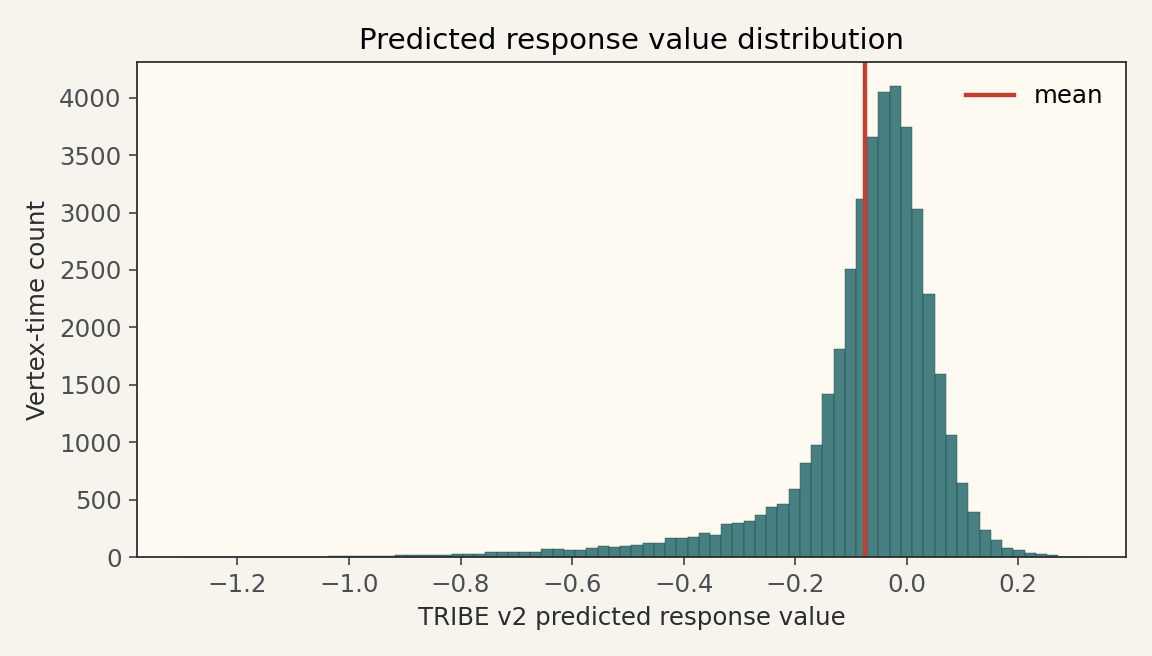
\includegraphics[width=0.88\linewidth]{figures/tribe_response_distribution.png}
  \caption{Distribution of predicted response values across both retained
  segments and all \responsevertices{} vertices.}
  \label{fig:distribution}
\end{figure}

\begin{figure}[ht]
  \centering
  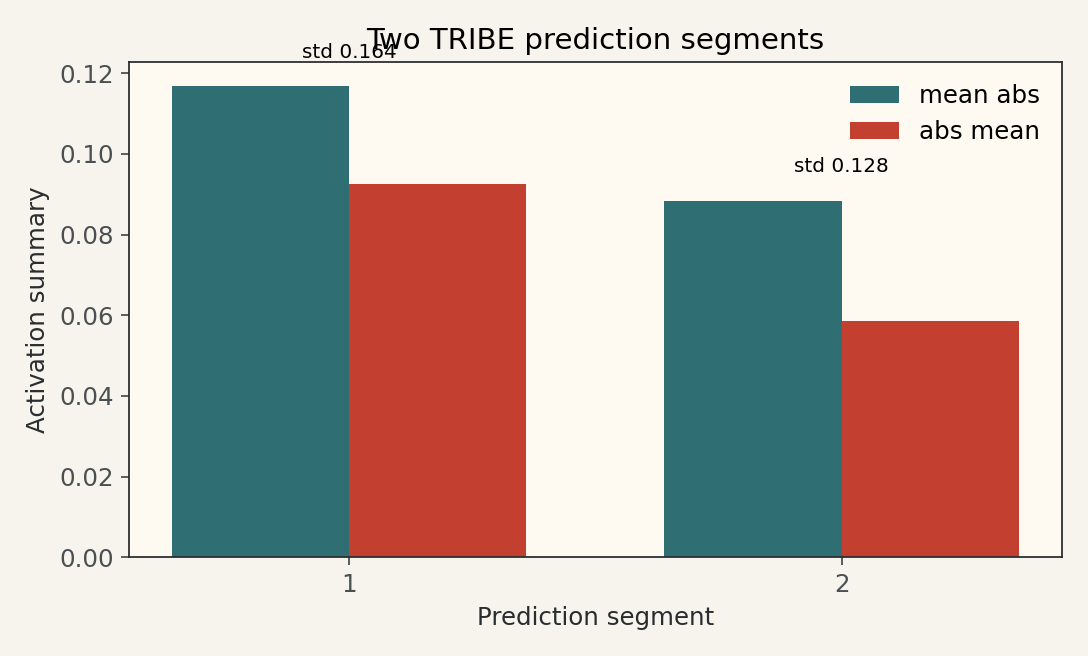
\includegraphics[width=0.88\linewidth]{figures/tribe_timepoint_summary.png}
  \caption{Two retained \tribe{} prediction segments. Bars summarize mean
  absolute predicted response and absolute mean response; labels show segment
  standard deviation.}
  \label{fig:segments}
\end{figure}

\subsection{Vertex-index brain schematic}

TRIBE's public documentation says predictions live on fsaverage5 at roughly
20k vertices \cite{tribev2repo}. Surface-based coordinate systems such as
FreeSurfer's fsaverage family derive from cortical-surface registration methods
designed to align folded cortical geometry across subjects
\cite{fischl1999surface,freesurferfsaverage}. A true anatomical rendering would
therefore require the matching surface coordinates or an atlas/annotation file.
This run artifact has neither.

The added brain diagram consequently uses a conservative schematic label:
\emph{fsaverage5 vertex-index schematic}. The \responsevertices{} response
values are split into two \hemivertices{}-value halves and labeled left/right
only as an index convention. Without the matching \tribe{} output
specification, surface coordinates, or annotation files, the split should not
be interpreted as independently verified hemispheric anatomy. Each half is
deterministically projected into a two-dimensional cortical silhouette. Color
encodes mean absolute predicted response across the two retained model output
segments. The figure highlights a small number of high-amplitude indices for
visual QA, but it does not assign anatomical areas or ROIs.

\begin{figure}[ht]
  \centering
  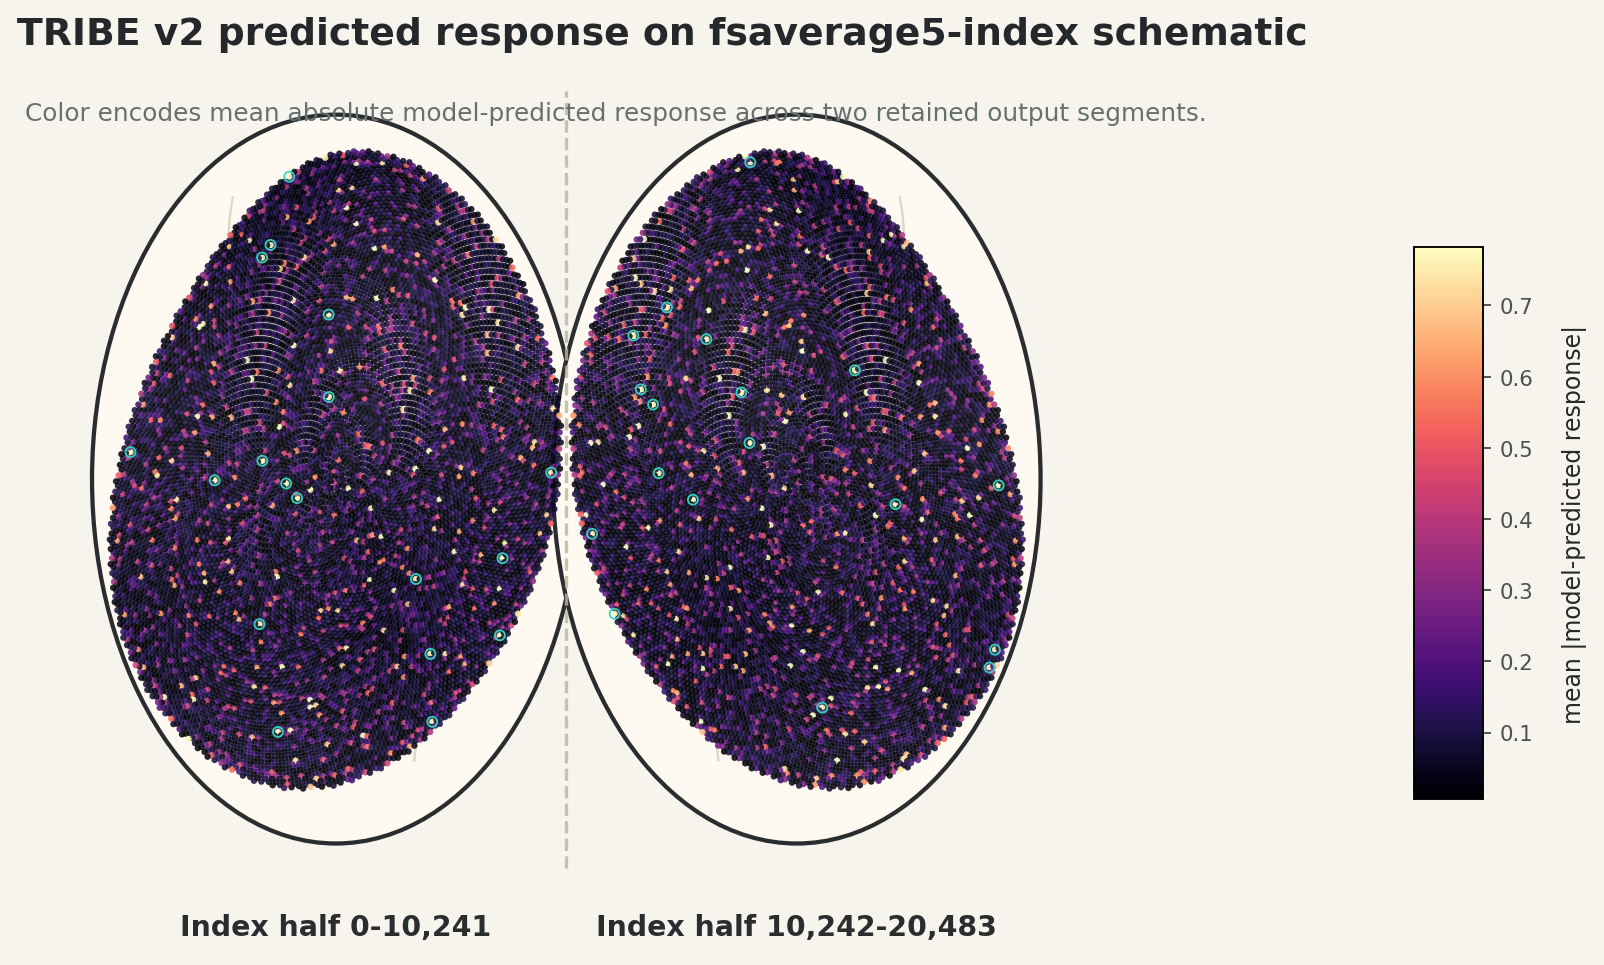
\includegraphics[width=\linewidth]{figures/tribe_brain_schematic.png}
  \caption{Vertex-index brain schematic. The first half of the
  \responsevertices{} vector is drawn as one hemisphere-shaped index map and
  the second half as the other by convention. This is a review diagram for
  orientation and QA, not a subject-specific anatomical registration, ROI
  atlas, or biological hemispheric analysis.}
  \label{fig:brain-schematic}
\end{figure}

\begin{table}[ht]
  \centering
  \caption{Brain-schematic metadata copied and normalized from the run-local
  schematic metadata file.}
  \label{tab:brain-metadata}
  \begin{tabular}{ll}
    \toprule
    Field & Value \\
    \midrule
    Schematic type & \texttt{fsaverage5\_vertex\_index\_schematic} \\
    First-half index range & 0--10{,}241 \\
    Second-half index range & 10{,}242--20{,}483 \\
    First-half mean absolute predicted response & 0.102728 \\
    Second-half mean absolute predicted response & 0.102612 \\
    First-half maximum absolute predicted response & 1.001841 \\
    Second-half maximum absolute predicted response & 1.078459 \\
    Color scale 2nd percentile & 0.006217 \\
    Color scale 99.5th percentile & 0.781990 \\
    \bottomrule
  \end{tabular}
\end{table}

\section{Results}

The result is intentionally small. The run demonstrates that the local harness can
prepare generated video stimuli, load the cached \tribe{} checkpoint, extract
video features, produce one structurally valid model-predicted response, and
validate the artifact layout. It also provides a concrete visualization path
that preserves caveats in the figure caption and metadata.

The response summary is finite and internally serializable. The mean absolute
predicted response for the retained stimulus is \meanabs{}. The two index-half
means are 0.102728 and 0.102612; these are serialization summaries, not
evidence of biological hemispheric symmetry. With only one completed model
prediction, pairwise response similarity is undefined and latent-component
analysis is correctly marked as insufficient-samples in the run metrics.

\begin{figure}[ht]
  \centering
  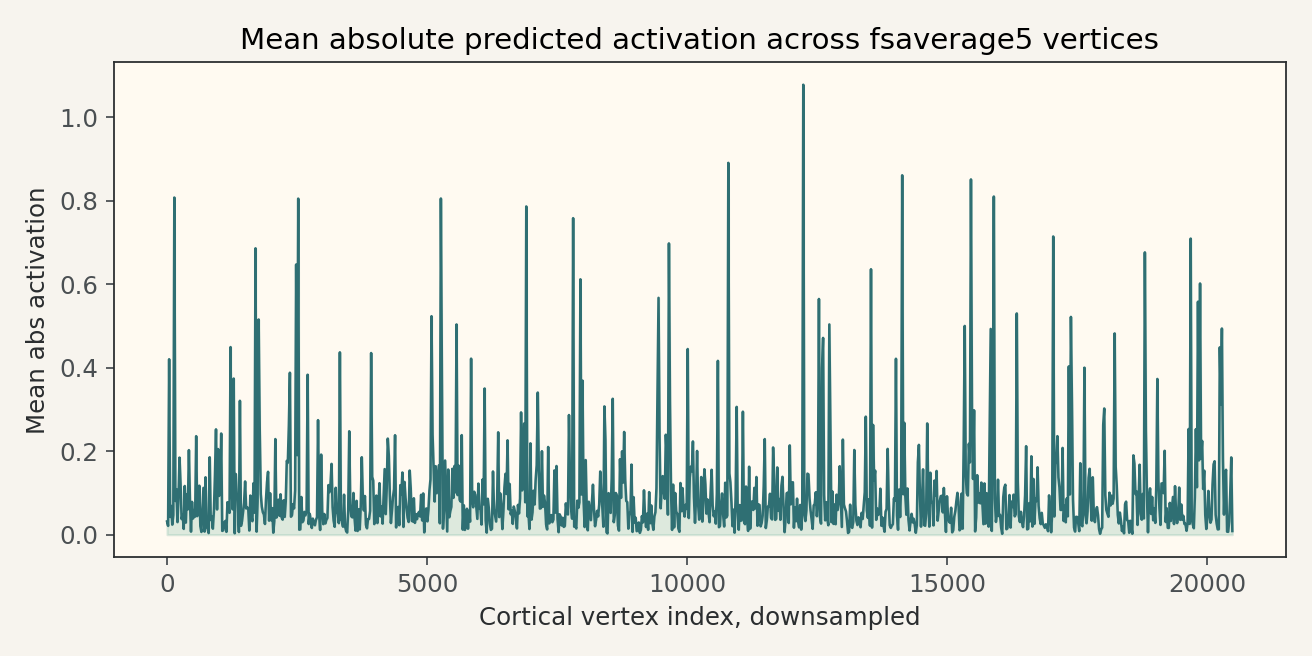
\includegraphics[width=0.96\linewidth]{figures/tribe_vertex_profile.png}
  \caption{Mean absolute predicted response by downsampled vertex index. This
  figure is useful for detecting gross serialization or plotting errors, but it
  is not an anatomical ROI summary.}
  \label{fig:vertex-profile}
\end{figure}

\begin{figure}[ht]
  \centering
  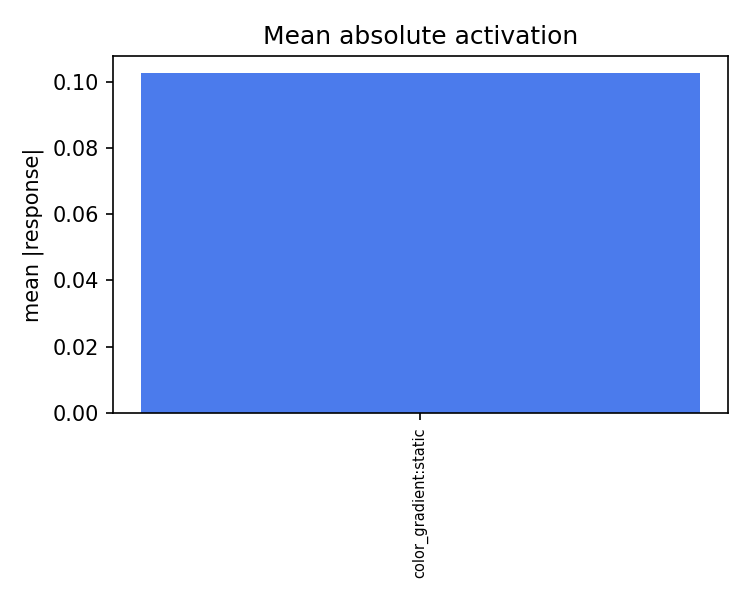
\includegraphics[width=0.88\linewidth]{figures/mean_abs_activation.png}
  \caption{Repository-generated mean absolute predicted-response summary for
  the one completed \tribe{} model prediction.}
  \label{fig:mean-abs}
\end{figure}

\section{Discussion}

The main value of this run is methodological. It establishes an end-to-end
local path from generated stimulus through \tribe{} inference, artifact
validation, HTML visualization, and LaTeX manuscript reporting. Because the
first-suite run is capped at one prediction, it is cheap enough to repeat on a
well-equipped workstation while still exercising the real model backend.

The brain schematic fills an immediate review need: it lets a reader see how a
\responsevertices{}-length cortical vector is being split and displayed. It
does not establish biological plausibility, hemispheric symmetry, or ROI
mapping. The correct next step for anatomical reporting is
to add the matching fsaverage5 surface coordinates and atlas annotations as
declared, versioned inputs, then derive ROI summaries from those files. Until
that is done, the diagram should remain labeled as a vertex-index schematic.

\section{Limitations}

This preprint has strong limitations by design. First, the values are
model-predicted average-subject fMRI-like responses, not measured neural
activity. Second, the experiment reports one completed prediction, so it cannot
support comparisons among stimulus families, statistical inference, or latent
network analysis. Third, the brain diagram is not an anatomical registration:
no fsaverage5 coordinate file, FreeSurfer subject, surface triangles, or ROI
annotation was present in the run artifact. Fourth, the response is based on a
generated synthetic visual stimulus and should not be generalized to natural
image responses. Fifth, the public \tribe{} weights and software have their own
non-commercial licensing constraints \cite{tribev2hf,tribev2repo}. Sixth,
local inference speed depends on cached model assets and hardware; this run
encoded four video feature batches in several minutes on the local machine.

\section{Reproducibility}

The run was produced from repository commit \runcommit{}. The manuscript branch
is later because it adds this preprint and prior BOLD5000 preprint
infrastructure. The experiment seed is 20260508. Table~\ref{tab:provenance}
records the run and model provenance needed to audit the artifact.

\begin{table}[ht]
  \centering
  \caption{Provenance identifiers for the source run and local model assets.}
  \label{tab:provenance}
  \begin{tabular}{p{0.28\linewidth}p{0.64\linewidth}}
    \toprule
    Field & Value \\
    \midrule
    Run config SHA-256 & \confighash{} \\
    Response archive SHA-256 & \responsehash{} \\
    Hugging Face snapshot &
      \provenancehash{f894e783020944dcd96e5568550afe2aa9743f9f} \\
    \texttt{best.ckpt} SHA-256 &
      \provenancehash{9c79ffff6b642b7b0c71d558c935fb3fa33f2788bfb509feead94fafbba2f321} \\
    \texttt{config.yaml} SHA-256 &
      \provenancehash{a17212a257dfd91424e20a5fa8640d107fbbf79e842b6b2d72d17d24399dc9ef} \\
    \bottomrule
  \end{tabular}
\end{table}

The active Python environment used Python 3.12.13 with
\pkg{braindough==0.1.0}, \pkg{tribev2==0.1.0}, \pkg{torch==2.6.0},
\pkg{neuralset==0.0.2}, \pkg{numpy==2.2.6}, \pkg{pandas==3.0.2},
\pkg{imageio==2.37.3}, \pkg{imageio-ffmpeg==0.6.0}, and
\pkg{pillow==11.3.0}.

Structural artifact validation checks the presence and internal consistency of
manifest/config files, response metadata, response shapes, required tables,
checksums, reports, and finite artifact values. It does not test whether the
\tribe{} model is accurate, calibrated, or valid for any neuroscientific claim.

The experiment can be rerun from the repository root with:

\begin{verbatim}
just bootstrap
just storage-doctor
just run-tribe
just artifact-validate RUN_DIR=<new-run-dir>
\end{verbatim}

The manuscript PDF is built with:

\begin{verbatim}
just preprint-build docs/preprints/2026-05-16T233000Z-tribe-v2-schematic-response
\end{verbatim}

The committed manuscript directory contains only small derivative figures and
tables. The full run directory, model caches, and response archive remain under
\texttt{BRAINDOUGH\_HOME}. This separation keeps the repository reviewable
without losing reproducibility metadata.

\section{AI-Assisted Review}

ChatGPT Extended Pro was used through the browser for iterative critique of
scientific framing, overclaim risk, and manuscript structure. Its feedback was
treated as advisory. The final claims are restricted to primary sources and
the validated local run artifact.

\section{Conclusion}

A bounded \braindough{} \tribe{} run can produce a structurally valid
model-predicted response artifact and a reviewable brain-schematic
visualization without overclaiming anatomical registration. The result is a
practical template for future local in-silico experiments: keep real model runs
capped, preserve heavy artifacts outside the repository, commit small
derivatives, and label visualizations according to the spatial information
actually present.

\appendix

\section{Suite Summary}

\begin{table}[ht]
  \centering
  \caption{Stimuli and completed responses by suite.}
  \label{tab:suite-summary}
  \begin{tabular}{lrr}
    \toprule
    Suite & Stimuli & Responses \\
    \midrule
    image activation & 3 & 1 \\
    visual controls & 5 & 0 \\
    visual perturbations & 18 & 0 \\
    temporalization & 9 & 0 \\
    audio controls & 4 & 0 \\
    \bottomrule
  \end{tabular}
\end{table}

\section{Copied Artifact Files}

\begin{itemize}
  \item \texttt{tables/metrics.json}
  \item \texttt{tables/vertex\_index\_schematic\_metadata.json}
  \item \texttt{tables/response\_metrics.csv}
  \item \texttt{tables/stimuli.csv}
  \item \texttt{figures/tribe\_brain\_schematic.png}
  \item \texttt{figures/tribe\_response\_distribution.png}
  \item \texttt{figures/tribe\_timepoint\_summary.png}
  \item \texttt{figures/tribe\_vertex\_profile.png}
  \item \texttt{figures/mean\_abs\_activation.png}
  \item \texttt{figures/response\_similarity.png}
  \item \texttt{figures/color\_gradient.png}
\end{itemize}

\begin{thebibliography}{9}
\raggedright

\bibitem{dascoli2026foundation}
d'Ascoli, S., Rapin, J., Benchetrit, Y., Brooks, T., Begany, K., Raugel, J.,
Banville, H., and King, J.-R. A foundation model of vision, audition, and
language for in-silico neuroscience. \emph{arXiv preprint}
arXiv:2605.04326 (2026). \url{https://arxiv.org/abs/2605.04326}.

\bibitem{tribev2repo}
facebookresearch. \tribe{} source repository and README. GitHub (2026).
\url{https://github.com/facebookresearch/tribev2}.

\bibitem{tribev2hf}
AI at Meta. \texttt{facebook/tribev2} model files and license. Hugging Face
(2026). \url{https://huggingface.co/facebook/tribev2}.

\bibitem{fischl1999surface}
Fischl, B., Sereno, M. I., and Dale, A. M. Cortical surface-based
analysis. II: Inflation, flattening, and a surface-based coordinate system.
\emph{NeuroImage} 9(2), 195--207 (1999). doi:10.1006/nimg.1998.0396.

\bibitem{freesurferfsaverage}
FreeSurfer Wiki. FsAverage. \url{https://freesurfer.net/fswiki/FsAverage}.

\end{thebibliography}

\end{document}
